\section{Design}
Sparkling Water is designed to be executed as a regular Spark application. It provides a way to initialize H2O services on each node in the Spark cluster and access data stored in data structures of Spark and H2O.

Since Sparkling Water is primarily designed as Spark application, it is launched
inside a Spark executor, which is created after application submission. At this
point, H2O starts services, including distributed K/V store and memory manager, and orchestrates them into a cloud. The topology of the created cloud matches the topology of the underlying Spark cluster exactly.

\begin{figure}[h]
	\centering
	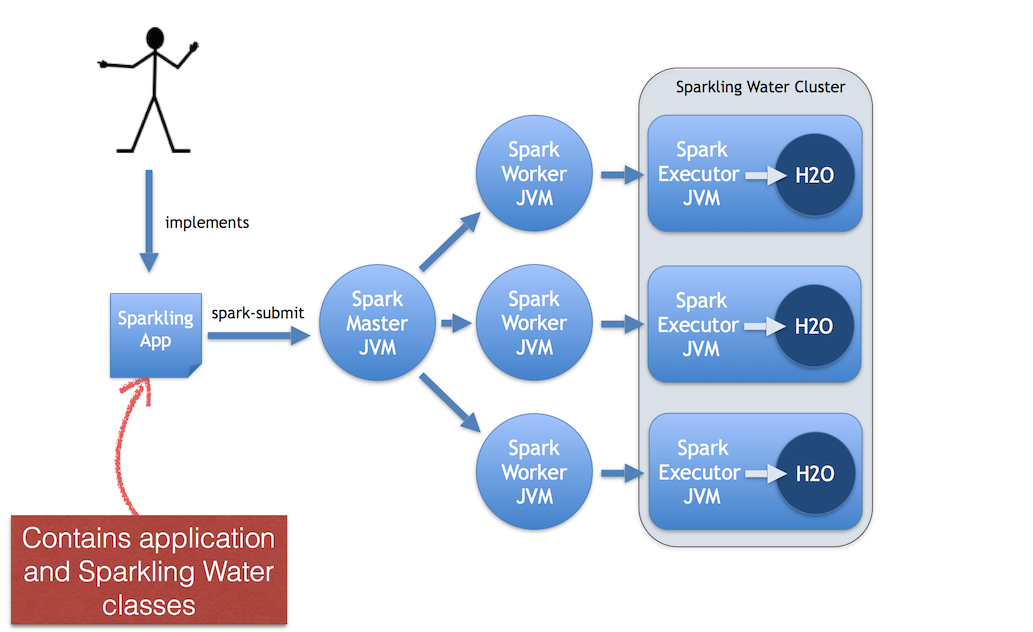
\includegraphics[width=\textwidth]{sw/images/Topology.png}
	\caption{Sparkling Water design. The scenario depicts deployment of Sparkling Water application to standalone Spark cluster.}
\end{figure}


\subsection{Data Sharing between Spark and H2O}

Sparkling Water enables transformation between different types of RDDs and H2O's H2OFrame, and vice versa.

When converting from H2OFrame to RDD, a wrapper is created around the H2O H2OFrame to provide an RDD-like API. In this case, no data is duplicated; instead, the data is served directly from then underlying H2OFrame.

Converting in the opposite direction (from RDD to H2OFrame) introduces data duplication, since it transfers data from RDD storage into H2OFrame. However, data stored in H2OFrame is heavily compressed.

\subsection{Provided Primitives}

\begin{table}
\centering
\begin{tabularx}{\textwidth}{l l p{5.2cm}}
\toprule
Concept & API Representation & Description \\
\midrule
H2O context & \texttt{H2OContext}\footnote{Fullname of class is \texttt{org.apache.spark.h2o.H2OContext}} & Holds
H2O state and provides primitives to publish \texttt{RDD} as \texttt{H2OFrame} and
vice versa. It follows design principles of Spark primitives such as
\texttt{SparkContext} or \texttt{SQLContext} \\  \addlinespace

H2O entry point & \texttt{H2O}\footnote{Fullname of class is \texttt{water.H2Ot}} & Represents the entry point for accessing
H2O services. It holds information about running H2O services including a list of
nodes and the status of distributed K/V datastore. \\  \addlinespace

H2O Frame & \texttt{H2OFrame}\footnote{Fullname of class is \texttt{water.fvec.H2OFrame}} & A data structure that
represents a table of values. The table is column-based and provides column and
row accessors. \\  \addlinespace

H2O Algorithm & package \texttt{hex} & Represents the H2O machine learning
algorithms library, including DeepLearning, GBM, GLM, RandomForest and other
algorithms. \\

\bottomrule
\end{tabularx}
\caption{Sparkling Water primitives}
\label{tab:primitives}
\end{table}

